\documentclass[11pt,a4paper]{article}

% ── Encoding & Language ──────────────────────────────────────────────
\usepackage[utf8]{inputenc}
\usepackage[T1]{fontenc}
\usepackage[english]{babel}

% ── Fonts ────────────────────────────────────────────────────────────
\usepackage{lmodern}
\usepackage{inconsolata}

% ── Layout ───────────────────────────────────────────────────────────
\usepackage[margin=2.5cm]{geometry}
\usepackage{parskip}
\usepackage{titlesec}
\usepackage{fancyhdr}
\usepackage{lastpage}

% ── Graphics & Diagrams ─────────────────────────────────────────────
\usepackage{tikz}
\usetikzlibrary{
  arrows.meta,
  positioning,
  shapes.geometric,
  shapes.multipart,
  fit,
  calc,
  decorations.pathreplacing,
  backgrounds,
  matrix
}
\usepackage{pgfplots}
\pgfplotsset{compat=1.18}

% ── Tables ───────────────────────────────────────────────────────────
\usepackage{booktabs}
\usepackage{tabularx}
\usepackage{multirow}
\usepackage{array}
\usepackage{colortbl}

% ── Code Listings ────────────────────────────────────────────────────
\usepackage{listings}
\usepackage{xcolor}

% ── Misc ─────────────────────────────────────────────────────────────
\usepackage{enumitem}
\usepackage{hyperref}
\usepackage{tcolorbox}
\tcbuselibrary{skins,breakable}
\usepackage{amsmath}
\usepackage{amssymb}
\usepackage{pifont}
\usepackage[normalem]{ulem}

% ── Colors ───────────────────────────────────────────────────────────
\definecolor{kernel}{RGB}{41,65,122}
\definecolor{user}{RGB}{52,152,72}
\definecolor{hw}{RGB}{180,60,40}
\definecolor{ipc}{RGB}{160,100,200}
\definecolor{capcolor}{RGB}{200,140,30}
\definecolor{bg}{RGB}{245,245,250}
\definecolor{codebg}{RGB}{248,248,252}
\definecolor{accent}{RGB}{41,65,122}
\definecolor{codegreen}{RGB}{40,160,60}
\definecolor{codegray}{RGB}{128,128,128}
\definecolor{codeblue}{RGB}{30,80,180}

% ── Listings Style ───────────────────────────────────────────────────
\lstdefinestyle{rust}{
  language=C,
  basicstyle=\ttfamily\small,
  backgroundcolor=\color{codebg},
  keywordstyle=\color{codeblue}\bfseries,
  stringstyle=\color{codegreen},
  commentstyle=\color{codegray}\itshape,
  numbers=left,
  numberstyle=\tiny\color{codegray},
  numbersep=8pt,
  frame=single,
  rulecolor=\color{codegray!30},
  breaklines=true,
  tabsize=4,
  showstringspaces=false,
  morekeywords={fn,let,mut,pub,struct,enum,impl,const,static,use,mod,
    self,Self,crate,super,unsafe,extern,async,await,where,
    u8,u16,u32,u64,usize,i64,bool,Option,Some,None,Result},
  literate={->}{{$\rightarrow$}}2 {=>}{{$\Rightarrow$}}2,
}
\lstset{style=rust}

% ── tcolorbox Styles ─────────────────────────────────────────────────
\newtcolorbox{principalbox}[1]{
  colback=kernel!5,
  colframe=kernel,
  fonttitle=\bfseries\sffamily,
  title=#1,
  arc=2mm,
  boxrule=0.8pt,
  breakable
}

\newtcolorbox{designbox}[1]{
  colback=user!5,
  colframe=user!80!black,
  fonttitle=\bfseries\sffamily,
  title=#1,
  arc=2mm,
  boxrule=0.8pt,
  breakable
}

\newtcolorbox{warningbox}[1]{
  colback=hw!5,
  colframe=hw,
  fonttitle=\bfseries\sffamily,
  title=#1,
  arc=2mm,
  boxrule=0.8pt,
  breakable
}

% ── Header/Footer ────────────────────────────────────────────────────
\pagestyle{fancy}
\fancyhf{}
\fancyhead[L]{\small\sffamily\color{accent} sotX Architecture}
\fancyhead[R]{\small\sffamily\color{accent} v0.1.0}
\fancyfoot[C]{\small\sffamily\thepage\ / \pageref{LastPage}}
\renewcommand{\headrulewidth}{0.4pt}
\renewcommand{\footrulewidth}{0.2pt}

% ── Title Formatting ─────────────────────────────────────────────────
\titleformat{\section}
  {\Large\bfseries\sffamily\color{accent}}
  {\thesection}{1em}{}[\vspace{-0.5em}\rule{\textwidth}{0.4pt}]

\titleformat{\subsection}
  {\large\bfseries\sffamily\color{accent!80}}
  {\thesubsection}{1em}{}

\titleformat{\subsubsection}
  {\normalsize\bfseries\sffamily\color{accent!60}}
  {\thesubsubsection}{1em}{}

% ── Checkmark / Cross ────────────────────────────────────────────────
\newcommand{\cmark}{\ding{51}}
\newcommand{\xmark}{\ding{55}}

% ═════════════════════════════════════════════════════════════════════
\begin{document}

% ── Title Page ───────────────────────────────────────────────────────
\begin{titlepage}
\centering
\vspace*{3cm}

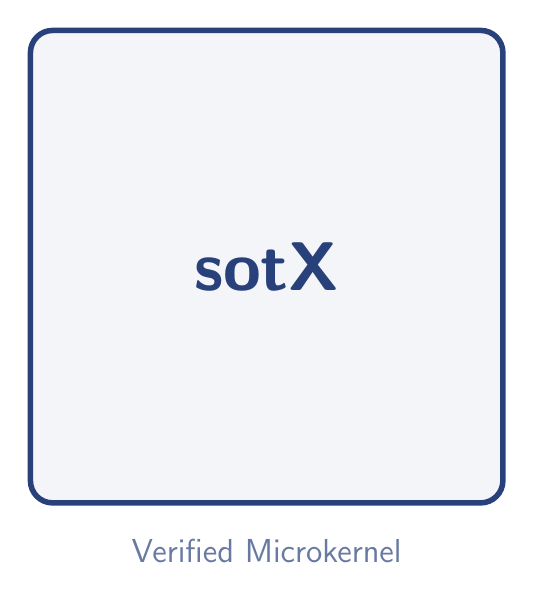
\begin{tikzpicture}
  \node[draw=kernel, line width=2pt, rounded corners=8pt,
        minimum width=6cm, minimum height=6cm, fill=kernel!5] (logo) {};
  \node[font=\fontsize{48}{48}\selectfont\bfseries\sffamily\color{kernel}]
    at (logo.center) {sotX};
  \node[font=\large\sffamily\color{kernel!70}, below=3mm]
    at (logo.south) {Verified Microkernel};
\end{tikzpicture}

\vspace{2cm}

{\Huge\bfseries\sffamily Architecture Document}

\vspace{0.5cm}

{\Large\sffamily\color{accent!70} Philosophy, Design \& Implementation}

\vspace{2cm}

{\large\sffamily
Version 0.1.0\\[0.5em]
March 2026
}

\vfill

{\small\sffamily\color{gray}
Microkernel + Selective Exokernel Bypass\\
Rust \textbullet{} Capability Security \textbullet{} Zero-Copy IPC \textbullet{} Formal Verification
}
\end{titlepage}

% ── Table of Contents ────────────────────────────────────────────────
\tableofcontents
\newpage

% ═════════════════════════════════════════════════════════════════════
\section{Philosophy: A Third Way}
% ═════════════════════════════════════════════════════════════════════

Operating systems have traditionally followed two opposing philosophies:

\begin{itemize}[leftmargin=2em]
  \item \textbf{Microkernels} (seL4, L4, Minix3): The kernel abstracts and mediates.
        Services ask the kernel for permission to do anything.
  \item \textbf{Exokernels} (MIT Exokernel, Unikernels): The kernel abstracts nothing ---
        it exposes raw hardware and lets applications manage their own resources.
\end{itemize}

sotX is neither. It is a \textbf{verified microkernel with selective exokernel bypass}.

\begin{principalbox}{The Core Idea}
The kernel is a formally verified microkernel managing exactly \textbf{five primitives}.
Virtual memory is handled by a \textit{userspace} server.
Applications that need maximum performance (databases, ML inference) can
\textit{bypass} the standard memory server and manage their own physical frames
directly --- as long as the kernel can verify they own those frames through capabilities.

\textbf{The kernel guarantees isolation, not policy.}
\end{principalbox}

This creates a spectrum: most applications use the standard VMM server and
get the safety of managed memory. Performance-critical applications opt out
and get raw hardware access --- but only to resources they hold capabilities for.

\subsection{Why Verification Matters}

Rust eliminates memory errors, but not logic errors. A scheduler written in Rust
can be memory-safe and still deadlock. A capability check can be memory-safe
and still have an off-by-one that grants too much access.

For a kernel of $\sim$10K lines, formal verification is tractable. seL4 proved it:
you can mathematically guarantee that the kernel never dereferences a null pointer,
never overflows a buffer, and that capability enforcement is correct.

\begin{center}
\begin{tabular}{lll}
\toprule
\textbf{Layer} & \textbf{Tool} & \textbf{Guarantee} \\
\midrule
Kernel          & Rust + Verus/Prusti     & Memory safety + functional correctness \\
Critical services & Rust + TLA+/Spin     & No deadlocks, liveness, fairness \\
Drivers/services  & Rust + fuzzing       & Memory safety + empirical robustness \\
\bottomrule
\end{tabular}
\end{center}

The 70\% figure (Microsoft/Google) covers memory bugs that Rust eliminates.
The remaining 30\% are logic bugs --- attacked with formal verification in the kernel
and contained by capability isolation everywhere else.

% ═════════════════════════════════════════════════════════════════════
\section{Architecture Overview}
% ═════════════════════════════════════════════════════════════════════

\begin{center}
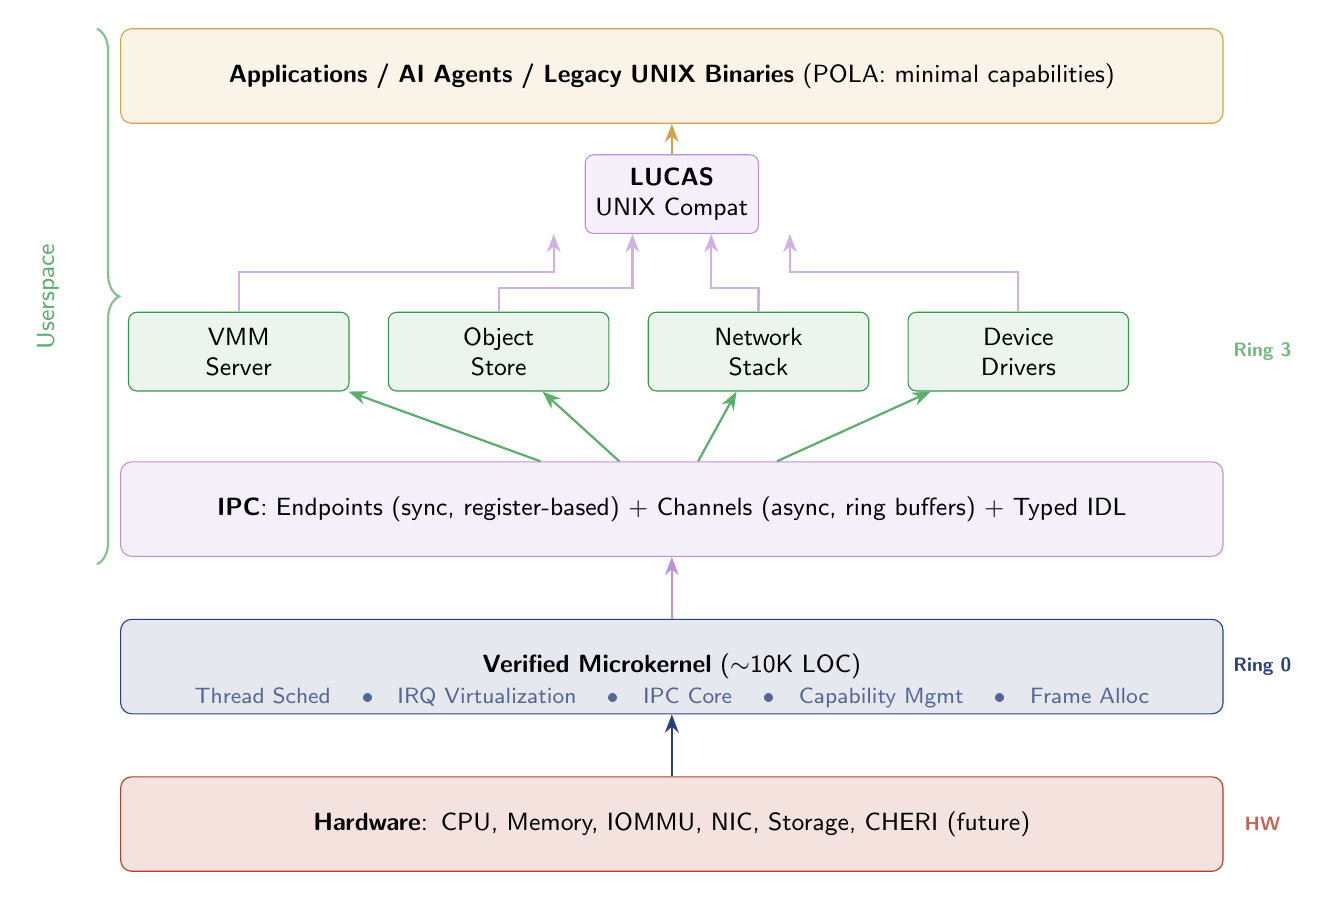
\begin{tikzpicture}[
  every node/.style={font=\sffamily\small},
  layer/.style={draw, rounded corners=4pt, minimum width=14cm, minimum height=1.2cm,
                text width=13cm, align=center},
  svc/.style={draw, rounded corners=3pt, minimum width=2.8cm, minimum height=1cm,
              align=center, fill=white},
  >=Stealth
]

% ── Hardware ──
\node[layer, fill=hw!15, draw=hw] (hw) at (0, 0)
  {\textbf{Hardware}: CPU, Memory, IOMMU, NIC, Storage, CHERI (future)};

% ── Kernel ──
\node[layer, fill=kernel!12, draw=kernel] (kern) at (0, 2)
  {\textbf{Verified Microkernel} ($\sim$10K LOC)};

\node[font=\sffamily\footnotesize, text=kernel!80] at (0, 1.6)
  {Thread Sched \quad\textbullet\quad IRQ Virtualization \quad\textbullet\quad
   IPC Core \quad\textbullet\quad Capability Mgmt \quad\textbullet\quad Frame Alloc};

% ── IPC Layer ──
\node[layer, fill=ipc!10, draw=ipc!70] (ipc) at (0, 4)
  {\textbf{IPC}: Endpoints (sync, register-based) + Channels (async, ring buffers) + Typed IDL};

% ── Services ──
\node[svc, fill=user!10, draw=user] (vmm) at (-5.5, 6) {VMM\\Server};
\node[svc, fill=user!10, draw=user] (fs)  at (-2.2, 6) {Object\\Store};
\node[svc, fill=user!10, draw=user] (net) at (1.1, 6) {Network\\Stack};
\node[svc, fill=user!10, draw=user] (dev) at (4.4, 6) {Device\\Drivers};

% ── LUCAS ──
\node[svc, fill=ipc!10, draw=ipc!70, minimum width=2.2cm] (lucas) at (0, 8)
  {\textbf{LUCAS}\\UNIX Compat};

% ── Applications ──
\node[layer, fill=capcolor!10, draw=capcolor!80] (apps) at (0, 9.5)
  {\textbf{Applications / AI Agents / Legacy UNIX Binaries} (POLA: minimal capabilities)};

% ── Arrows ──
\draw[->, thick, kernel] (hw) -- (kern);
\draw[->, thick, ipc!70] (kern) -- (ipc);
\draw[->, thick, user!80] (ipc) -- (vmm);
\draw[->, thick, user!80] (ipc) -- (fs);
\draw[->, thick, user!80] (ipc) -- (net);
\draw[->, thick, user!80] (ipc) -- (dev);

% Services → LUCAS
\draw[->, thick, ipc!50] (vmm.north) -- ++(0,0.5) -| ([xshift=-1.5cm]lucas.south);
\draw[->, thick, ipc!50] (fs.north) -- ++(0,0.3) -| ([xshift=-0.5cm]lucas.south);
\draw[->, thick, ipc!50] (net.north) -- ++(0,0.3) -| ([xshift=0.5cm]lucas.south);
\draw[->, thick, ipc!50] (dev.north) -- ++(0,0.5) -| ([xshift=1.5cm]lucas.south);

% LUCAS + Services → Apps
\draw[->, thick, capcolor!80] (lucas.north) -- (apps.south);

% ── Ring labels ──
\node[font=\sffamily\scriptsize\bfseries, text=hw!80] at (7.5, 0) {HW};
\node[font=\sffamily\scriptsize\bfseries, text=kernel] at (7.5, 2) {Ring 0};
\node[font=\sffamily\scriptsize\bfseries, text=user!70] at (7.5, 6) {Ring 3};

% ── Bracket for userspace ──
\draw[decorate, decoration={brace, amplitude=8pt, mirror},
      thick, user!60]
  (-7.3, 3.3) -- (-7.3, 10.1)
  node[midway, left=10pt, font=\sffamily\small, text=user!80, rotate=90, anchor=south]
  {Userspace};

\end{tikzpicture}
\end{center}

\subsection{What Lives Where}

\begin{center}
\begin{tabularx}{\textwidth}{lXl}
\toprule
\textbf{Component} & \textbf{Responsibility} & \textbf{Ring} \\
\midrule
Thread scheduler & Preemptive scheduling between domains & 0 \\
IRQ virtualizer & Route hardware interrupts to userspace & 0 \\
IPC core & Endpoint rendezvous, channel setup & 0 \\
Capability manager & CDT, delegation, revocation & 0 \\
Frame allocator & Physical memory allocation & 0 \\
\midrule
VMM server & Page tables, virtual memory policy & 3 \\
Object store & Transactional storage, OIDs & 3 \\
Network stack & TCP/IP, socket API & 3 \\
Device drivers & Hardware I/O, DMA & 3 \\
Scheduling domains & Intra-domain thread scheduling & 3 \\
\bottomrule
\end{tabularx}
\end{center}

% ═════════════════════════════════════════════════════════════════════
\section{The Five Kernel Primitives}
% ═════════════════════════════════════════════════════════════════════

The kernel implements exactly five primitives. Everything else --- filesystems,
networking, device drivers, virtual memory policy --- runs in userspace.

\begin{center}
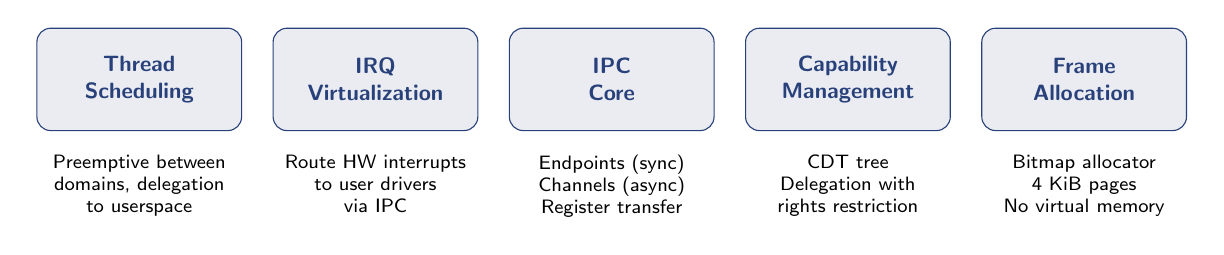
\begin{tikzpicture}[
  prim/.style={draw=kernel, fill=kernel!10, rounded corners=5pt,
               minimum width=2.6cm, minimum height=1.3cm, align=center,
               font=\sffamily\footnotesize\bfseries, text=kernel},
  desc/.style={font=\sffamily\scriptsize, text width=2.6cm, align=center},
  >=Stealth
]

\node[prim] (sched) at (0, 0)    {Thread\\Scheduling};
\node[prim] (irq)   at (3, 0)    {IRQ\\Virtualization};
\node[prim] (ipc)   at (6, 0)    {IPC\\Core};
\node[prim] (cap)   at (9, 0)    {Capability\\Management};
\node[prim] (frame) at (12, 0)   {Frame\\Allocation};

\node[desc, below=5pt] at (sched.south) {Preemptive between\\domains, delegation\\to userspace};
\node[desc, below=5pt] at (irq.south)   {Route HW interrupts\\to user drivers\\via IPC};
\node[desc, below=5pt] at (ipc.south)   {Endpoints (sync)\\Channels (async)\\Register transfer};
\node[desc, below=5pt] at (cap.south)   {CDT tree\\Delegation with\\rights restriction};
\node[desc, below=5pt] at (frame.south) {Bitmap allocator\\4 KiB pages\\No virtual memory};

\end{tikzpicture}
\end{center}

\subsection{Primitive 1: Thread Scheduling}

The kernel scheduler is \textbf{preemptive} and \textbf{priority-based}. It schedules
\textit{between scheduling domains} --- coarse-grained decisions involving at most
dozens of entities. Within each domain, userspace implements its own scheduler
(cooperative green threads, work-stealing pools, dedicated cores, etc.).

\begin{designbox}{Why Hierarchical Scheduling?}
\begin{itemize}[leftmargin=1.5em]
  \item The kernel makes few, fast decisions (which domain gets the CPU).
  \item Domain-internal scheduling is specialized per workload.
  \item If a domain misbehaves (exceeds its quantum), the kernel preempts it.
  \item Most context switches happen \textit{within} a domain --- in userspace, with zero syscalls.
\end{itemize}
\end{designbox}

\begin{center}
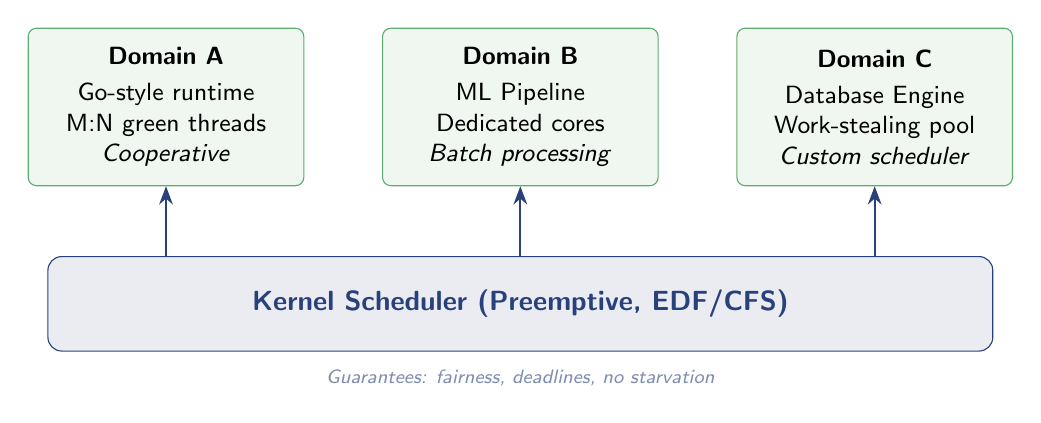
\begin{tikzpicture}[
  every node/.style={font=\sffamily\small},
  domainbox/.style={draw=user!80, fill=user!8, rounded corners=3pt,
                 minimum width=3.5cm, minimum height=2cm, align=center},
  ksched/.style={draw=kernel, fill=kernel!10, rounded corners=5pt,
                 minimum width=12cm, minimum height=1.2cm, align=center,
                 font=\sffamily\bfseries, text=kernel},
  >=Stealth
]

\node[ksched] (ks) at (0, 0)
  {Kernel Scheduler (Preemptive, EDF/CFS)};

\node[domainbox] (d1) at (-4.5, 2.5) {%
  \textbf{Domain A}\\[2pt]
  Go-style runtime\\
  M:N green threads\\
  \textit{Cooperative}
};

\node[domainbox] (d2) at (0, 2.5) {%
  \textbf{Domain B}\\[2pt]
  ML Pipeline\\
  Dedicated cores\\
  \textit{Batch processing}
};

\node[domainbox] (d3) at (4.5, 2.5) {%
  \textbf{Domain C}\\[2pt]
  Database Engine\\
  Work-stealing pool\\
  \textit{Custom scheduler}
};

\draw[->, thick, kernel] (ks.north -| d1) -- (d1.south);
\draw[->, thick, kernel] (ks.north) -- (d2.south);
\draw[->, thick, kernel] (ks.north -| d3) -- (d3.south);

\node[font=\sffamily\scriptsize\itshape, text=kernel!60, below=3pt] at (ks.south)
  {Guarantees: fairness, deadlines, no starvation};

\end{tikzpicture}
\end{center}

\subsection{Primitive 2: IRQ Virtualization}

Hardware interrupts are \textbf{not handled by the kernel} beyond acknowledging them.
Instead, the kernel delivers IRQ notifications to userspace driver threads via IPC endpoints.

\begin{enumerate}[leftmargin=2em]
  \item A driver registers for an IRQ: \texttt{sys\_irq\_register(irq\_cap, endpoint\_cap)}
  \item Hardware fires the IRQ $\rightarrow$ kernel handler sends notification to the endpoint
  \item Driver thread (blocked on \texttt{recv}) wakes up and handles the interrupt
  \item Driver acknowledges: \texttt{sys\_irq\_ack(irq\_cap)} $\rightarrow$ kernel unmasks the IRQ line
\end{enumerate}

\subsection{Primitive 3: IPC Core}

Two mechanisms, optimized for different use cases:

\begin{center}
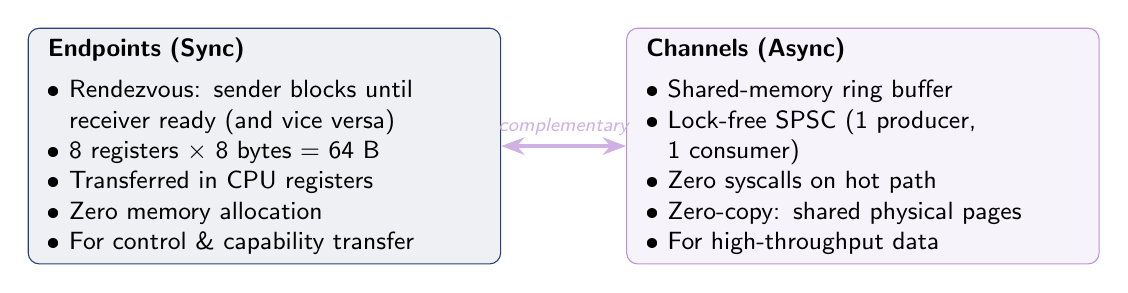
\begin{tikzpicture}[
  every node/.style={font=\sffamily\small},
  mech/.style={draw, rounded corners=4pt, minimum width=6cm, minimum height=2.5cm,
               align=left, text width=5.5cm},
  >=Stealth
]

\node[mech, fill=kernel!8, draw=kernel] (ep) at (-3.8, 0) {%
  \textbf{Endpoints (Sync)}\\[4pt]
  \textbullet{} Rendezvous: sender blocks until\\
  \phantom{\textbullet{}} receiver ready (and vice versa)\\
  \textbullet{} 8 registers $\times$ 8 bytes = 64 B\\
  \textbullet{} Transferred in CPU registers\\
  \textbullet{} Zero memory allocation\\
  \textbullet{} For control \& capability transfer
};

\node[mech, fill=ipc!8, draw=ipc!70] (ch) at (3.8, 0) {%
  \textbf{Channels (Async)}\\[4pt]
  \textbullet{} Shared-memory ring buffer\\
  \textbullet{} Lock-free SPSC (1 producer,\\
  \phantom{\textbullet{}} 1 consumer)\\
  \textbullet{} Zero syscalls on hot path\\
  \textbullet{} Zero-copy: shared physical pages\\
  \textbullet{} For high-throughput data
};

\draw[<->, very thick, ipc!50] (ep.east) -- (ch.west)
  node[midway, above, font=\sffamily\scriptsize\itshape] {complementary};

\end{tikzpicture}
\end{center}

\subsubsection{Endpoint Message Transfer}

When sender and receiver rendezvous, message registers are copied directly
between thread contexts during the context switch --- zero intermediate buffers:

\begin{center}
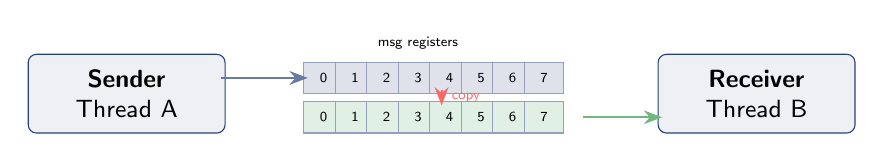
\begin{tikzpicture}[
  every node/.style={font=\sffamily\small},
  thread/.style={draw=kernel, fill=kernel!8, rounded corners=3pt,
                 minimum width=2.5cm, minimum height=1cm, align=center},
  reg/.style={draw=kernel!50, fill=white, minimum width=0.5cm, minimum height=0.4cm,
              font=\sffamily\tiny},
  >=Stealth
]

\node[thread] (sender) at (0, 0) {\textbf{Sender}\\Thread A};
\node[thread] (recver) at (8, 0) {\textbf{Receiver}\\Thread B};

% Registers
\foreach \i in {0,...,7} {
  \node[reg, fill=kernel!15] (sr\i) at (2.5 + \i*0.4, 0.2) {\i};
  \node[reg, fill=user!15]   (rr\i) at (2.5 + \i*0.4, -0.3) {\i};
}

\node[font=\sffamily\tiny, above=1pt] at (sr3.north) {msg registers};

\draw[->, thick, kernel!70] (1.2, 0.2) -- (2.3, 0.2);
\draw[->, thick, user!70] (5.8, -0.3) -- (6.8, -0.3);

\draw[->, thick, red!60, dashed] (4, 0.05) -- (4, -0.15)
  node[midway, right, font=\sffamily\tiny] {copy};

\end{tikzpicture}
\end{center}

\subsubsection{Channel Ring Buffer}

For bulk data transfer, shared-memory channels avoid syscalls entirely on the hot path:

\begin{center}
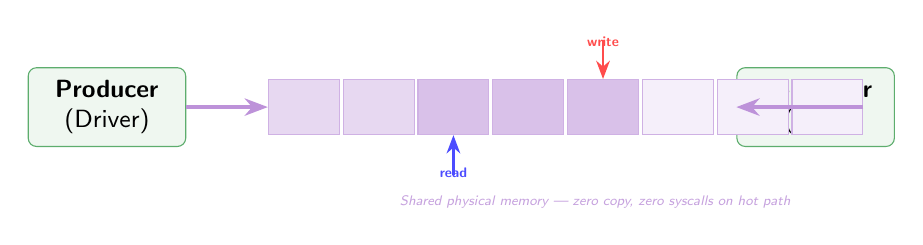
\begin{tikzpicture}[
  every node/.style={font=\sffamily\small},
  cell/.style={draw=ipc!50, minimum width=0.9cm, minimum height=0.7cm,
               font=\sffamily\tiny},
  >=Stealth
]

\node[draw=user!80, fill=user!8, rounded corners=3pt,
      minimum width=2cm, minimum height=1cm, align=center]
  (prod) at (-3, 0) {\textbf{Producer}\\(Driver)};

\node[draw=user!80, fill=user!8, rounded corners=3pt,
      minimum width=2cm, minimum height=1cm, align=center]
  (cons) at (6, 0) {\textbf{Consumer}\\(App)};

% Ring buffer cells
\foreach \i/\c in {0/ipc!25, 1/ipc!25, 2/ipc!40, 3/ipc!40, 4/ipc!40, 5/ipc!10, 6/ipc!10, 7/ipc!10} {
  \node[cell, fill=\c] (c\i) at (-0.5 + \i*0.95, 0) {};
}

\draw[->, very thick, ipc!70] (prod.east) -- (c0.west);
\draw[->, very thick, ipc!70] (c7.east) -- (cons.west);

% Write pointer
\draw[->, thick, red!70] (c4.north) ++(0, 0.5) -- (c4.north)
  node[above=8pt, font=\sffamily\tiny\bfseries, text=red!70] {write};

% Read pointer
\draw[->, thick, blue!70] (c2.south) ++(0, -0.5) -- (c2.south)
  node[below=8pt, font=\sffamily\tiny\bfseries, text=blue!70] {read};

\node[font=\sffamily\tiny\itshape, text=ipc!60] at (3.2, -1.2)
  {Shared physical memory --- zero copy, zero syscalls on hot path};

\end{tikzpicture}
\end{center}

\subsection{Primitive 4: Capability Management}

Every kernel object is accessed through a \textbf{capability} --- an opaque handle
with associated rights. Processes never see raw pointers to kernel objects;
they see tokens that the kernel translates.

\subsubsection{Capability Derivation Tree (CDT)}

When a capability is \textit{delegated}, the kernel records the parent-child relationship
in a tree. Revoking a parent automatically invalidates all descendants:

\begin{center}
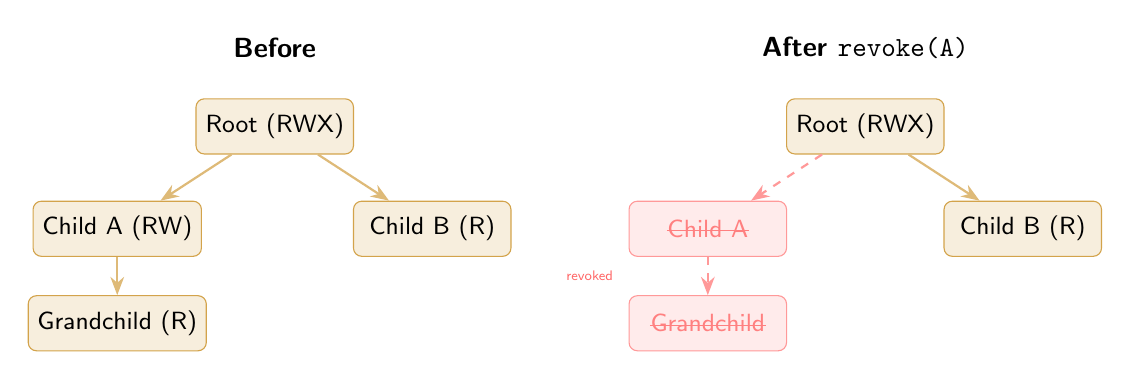
\begin{tikzpicture}[
  every node/.style={font=\sffamily\small},
  capnode/.style={draw=capcolor!80, fill=capcolor!15, rounded corners=3pt,
              minimum width=2cm, minimum height=0.7cm, align=center},
  dead/.style={draw=red!40, fill=red!8, rounded corners=3pt,
               minimum width=2cm, minimum height=0.7cm, align=center,
               text=red!50},
  >=Stealth
]

% Before revocation
\node[font=\sffamily\bfseries] at (-3.5, 3) {Before};

\node[capnode] (r) at (-3.5, 2)   {Root (RWX)};
\node[capnode] (a) at (-5.5, 0.7) {Child A (RW)};
\node[capnode] (b) at (-1.5, 0.7) {Child B (R)};
\node[capnode] (c) at (-5.5, -0.5) {Grandchild (R)};

\draw[->, thick, capcolor!60] (r) -- (a);
\draw[->, thick, capcolor!60] (r) -- (b);
\draw[->, thick, capcolor!60] (a) -- (c);

% After revocation
\node[font=\sffamily\bfseries] at (4, 3) {After \texttt{revoke(A)}};

\node[capnode] (r2) at (4, 2) {Root (RWX)};
\node[dead] (a2) at (2, 0.7) {\sout{Child A}};
\node[capnode] (b2) at (6, 0.7) {Child B (R)};
\node[dead] (c2) at (2, -0.5) {\sout{Grandchild}};

\draw[->, thick, red!40, dashed] (r2) -- (a2);
\draw[->, thick, capcolor!60] (r2) -- (b2);
\draw[->, thick, red!40, dashed] (a2) -- (c2);

\node[font=\sffamily\tiny, text=red!60] at (0.5, 0.1) {revoked};

\end{tikzpicture}
\end{center}

\subsubsection{Capability Types}

\begin{center}
\begin{tabular}{lll}
\toprule
\textbf{Type} & \textbf{Object} & \textbf{Rights} \\
\midrule
\texttt{Memory}   & Physical frame(s)   & Read, Write, Execute, Grant, Revoke \\
\texttt{Endpoint} & IPC endpoint        & Send, Receive, Grant \\
\texttt{Thread}   & Thread control      & Suspend, Resume, Destroy, Grant \\
\texttt{Irq}      & Hardware IRQ line   & Register, Ack, Grant \\
\texttt{IoPort}   & x86 I/O port range  & Read, Write, Grant \\
\bottomrule
\end{tabular}
\end{center}

\subsection{Primitive 5: Frame Allocation}

The kernel manages physical memory as 4\,KiB frames using a bitmap allocator.
Each bit represents one frame: 0 = free, 1 = allocated.

\begin{warningbox}{Critical Design Decision}
The kernel does \textbf{not} manage virtual memory (page tables, mappings).
That is the job of the userspace VMM server. The kernel only:
\begin{enumerate}[leftmargin=1.5em]
  \item Allocates/frees physical frames
  \item Verifies that \texttt{sys\_map()} calls reference frames the caller owns (via capability)
  \item Ensures kernel memory is never mapped to userspace
\end{enumerate}
This is what enables the exokernel bypass: a process with frame capabilities
can map memory however it wants, without going through the VMM.
\end{warningbox}

% ═════════════════════════════════════════════════════════════════════
\section{Security Model: Defense in Depth}
% ═════════════════════════════════════════════════════════════════════

sotX implements four layers of defense. Each layer catches what the layers
above it miss:

\begin{center}
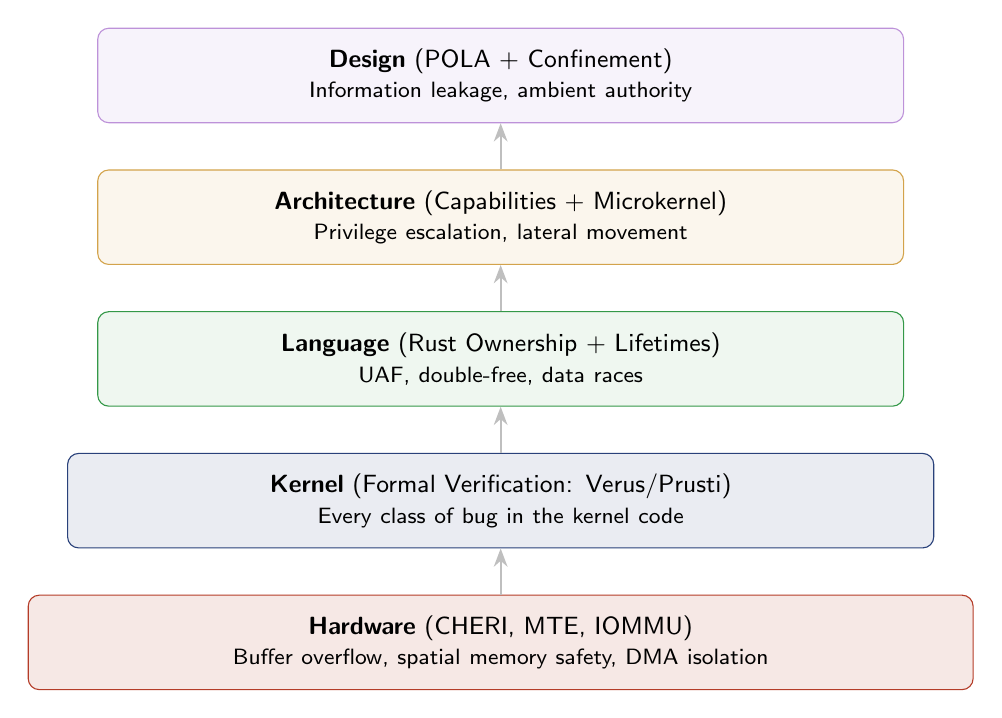
\begin{tikzpicture}[
  every node/.style={font=\sffamily\small},
  layer/.style={draw, rounded corners=4pt, minimum height=1.2cm,
                align=center, text width=10cm},
  >=Stealth
]

\node[layer, fill=hw!12, draw=hw, minimum width=12cm]
  (l1) at (0, 0)
  {\textbf{Hardware} (CHERI, MTE, IOMMU)\\
   \footnotesize Buffer overflow, spatial memory safety, DMA isolation};

\node[layer, fill=kernel!10, draw=kernel, minimum width=11cm]
  (l2) at (0, 1.8)
  {\textbf{Kernel} (Formal Verification: Verus/Prusti)\\
   \footnotesize Every class of bug in the kernel code};

\node[layer, fill=user!8, draw=user, minimum width=10cm]
  (l3) at (0, 3.6)
  {\textbf{Language} (Rust Ownership + Lifetimes)\\
   \footnotesize UAF, double-free, data races};

\node[layer, fill=capcolor!8, draw=capcolor!80, minimum width=9cm]
  (l4) at (0, 5.4)
  {\textbf{Architecture} (Capabilities + Microkernel)\\
   \footnotesize Privilege escalation, lateral movement};

\node[layer, fill=ipc!8, draw=ipc!70, minimum width=8cm]
  (l5) at (0, 7.2)
  {\textbf{Design} (POLA + Confinement)\\
   \footnotesize Information leakage, ambient authority};

% Arrows
\draw[->, thick, gray!50] (l1.north) -- (l2.south);
\draw[->, thick, gray!50] (l2.north) -- (l3.south);
\draw[->, thick, gray!50] (l3.north) -- (l4.south);
\draw[->, thick, gray!50] (l4.north) -- (l5.south);

\end{tikzpicture}
\end{center}

\subsection{Confinement}

A process can be launched with the guarantee that it \textbf{cannot leak information}
outside the capabilities it was given. This is essential for sandboxing untrusted code:
plugins, extensions, downloaded code.

The property is enforced structurally: if a process holds no \texttt{Send} capability
to any external endpoint, it physically cannot communicate with the outside world.
No ambient authority exists --- there are no global namespaces, no file paths
accessible without a capability, no implicit shared state.

\subsection{CHERI Integration (Future)}

ARM Morello implements CHERI --- Capability Hardware Enhanced RISC Instructions.
Instead of raw 64-bit pointers, CHERI uses 128-bit ``fat pointers'' carrying
bounds and permission metadata \textit{in hardware}. A buffer overflow doesn't just
get caught by software --- the CPU traps before the instruction executes.

\begin{center}
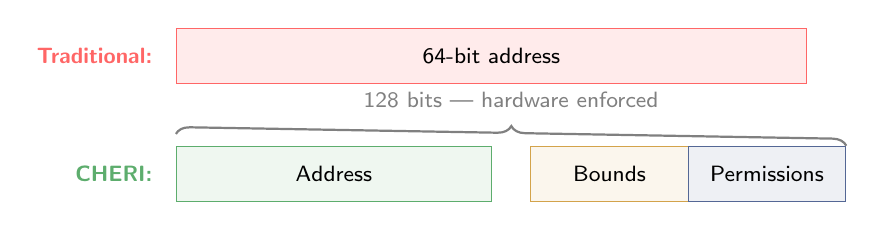
\begin{tikzpicture}[
  every node/.style={font=\sffamily\small},
  >=Stealth
]

% Traditional pointer
\node[draw=red!60, fill=red!8, minimum width=8cm, minimum height=0.7cm]
  (trad) at (0, 1.5) {};
\node[font=\sffamily\footnotesize] at (0, 1.5) {64-bit address};
\node[font=\sffamily\footnotesize\bfseries, text=red!60, left=5pt] at (trad.west) {Traditional:};

% CHERI pointer
\node[draw=user!80, fill=user!8, minimum width=4cm, minimum height=0.7cm]
  (addr) at (-2, 0) {};
\node[draw=capcolor!80, fill=capcolor!8, minimum width=2cm, minimum height=0.7cm]
  (bounds) at (1.5, 0) {};
\node[draw=kernel!80, fill=kernel!8, minimum width=2cm, minimum height=0.7cm]
  (perms) at (3.5, 0) {};

\node[font=\sffamily\footnotesize] at (-2, 0) {Address};
\node[font=\sffamily\footnotesize] at (1.5, 0) {Bounds};
\node[font=\sffamily\footnotesize] at (3.5, 0) {Permissions};
\node[font=\sffamily\footnotesize\bfseries, text=user!80, left=5pt] at (addr.west) {CHERI:};

\draw[decorate, decoration={brace, amplitude=5pt}, thick, gray]
  (addr.north west) ++(0, 0.15) -- (perms.north east |- addr.north) ++(0, 0.15)
  node[midway, above=8pt, font=\sffamily\footnotesize] {128 bits --- hardware enforced};

\end{tikzpicture}
\end{center}

% ═════════════════════════════════════════════════════════════════════
\section{Memory Model}
% ═════════════════════════════════════════════════════════════════════

\subsection{Physical Memory: Kernel Domain}

The kernel sees physical memory as a flat array of 4\,KiB frames. At boot,
the Limine bootloader provides a memory map, and the kernel builds a bitmap:

\begin{center}
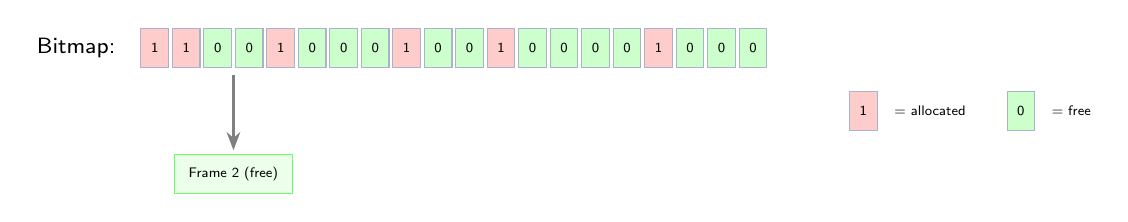
\begin{tikzpicture}[
  every node/.style={font=\sffamily},
  cell/.style={draw=kernel!40, minimum width=0.35cm, minimum height=0.5cm,
               font=\sffamily\tiny, inner sep=0},
  >=Stealth
]

% Bitmap row
\foreach \i/\v/\c in {
  0/1/red!20, 1/1/red!20, 2/0/green!20, 3/0/green!20, 4/1/red!20,
  5/0/green!20, 6/0/green!20, 7/0/green!20, 8/1/red!20, 9/0/green!20,
  10/0/green!20, 11/1/red!20, 12/0/green!20, 13/0/green!20, 14/0/green!20,
  15/0/green!20, 16/1/red!20, 17/0/green!20, 18/0/green!20, 19/0/green!20
} {
  \node[cell, fill=\c] at (\i*0.4, 0) {\v};
}

\node[font=\sffamily\footnotesize, left=5pt] at (-0.2, 0) {Bitmap:};

% Legend
\node[cell, fill=red!20] at (9, -0.8) {1};
\node[font=\sffamily\tiny, right=2pt] at (9.2, -0.8) {= allocated};
\node[cell, fill=green!20] at (11, -0.8) {0};
\node[font=\sffamily\tiny, right=2pt] at (11.2, -0.8) {= free};

% Arrow to frames
\draw[->, thick, gray] (2.5*0.4, -0.35) -- (2.5*0.4, -1.3);
\node[draw=green!60, fill=green!8, minimum width=1.5cm, minimum height=0.5cm,
      font=\sffamily\tiny] at (2.5*0.4, -1.6) {Frame 2 (free)};

\end{tikzpicture}
\end{center}

\subsection{Virtual Memory: Userspace Domain}

The kernel does \textbf{not} maintain page tables for user processes. Instead:

\begin{enumerate}[leftmargin=2em]
  \item The VMM server receives page fault notifications from the kernel
  \item It decides how to handle the fault (allocate, map, swap, deny)
  \item It calls \texttt{sys\_map(addr\_space\_cap, vaddr, frame\_cap, flags)} to install mappings
  \item The kernel verifies the capability and writes the page table entry
\end{enumerate}

\begin{center}
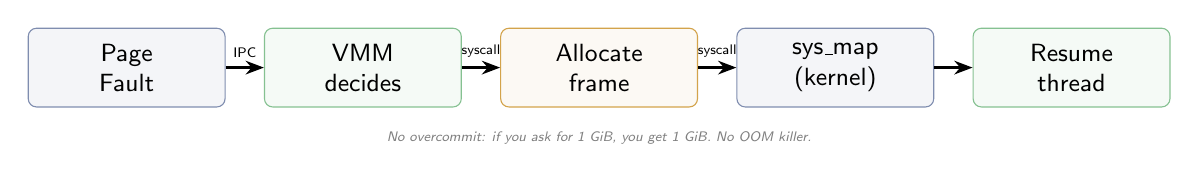
\begin{tikzpicture}[
  every node/.style={font=\sffamily\small},
  stepbox/.style={draw=kernel!60, fill=kernel!5, rounded corners=3pt,
               minimum width=2.5cm, minimum height=1cm, align=center},
  >=Stealth
]

\node[stepbox] (fault) at (0, 0) {Page\\Fault};
\node[stepbox, draw=user!60, fill=user!5] (vmm) at (3, 0) {VMM\\decides};
\node[stepbox, draw=capcolor!80, fill=capcolor!5] (alloc) at (6, 0) {Allocate\\frame};
\node[stepbox] (map) at (9, 0) {sys\_map\\(kernel)};
\node[stepbox, draw=user!60, fill=user!5] (resume) at (12, 0) {Resume\\thread};

\draw[->, thick] (fault) -- (vmm) node[midway, above, font=\sffamily\tiny] {IPC};
\draw[->, thick] (vmm) -- (alloc) node[midway, above, font=\sffamily\tiny] {syscall};
\draw[->, thick] (alloc) -- (map) node[midway, above, font=\sffamily\tiny] {syscall};
\draw[->, thick] (map) -- (resume);

\node[font=\sffamily\tiny\itshape, text=gray] at (6, -0.9)
  {No overcommit: if you ask for 1 GiB, you get 1 GiB. No OOM killer.};

\end{tikzpicture}
\end{center}

\subsection{Higher-Half Kernel}

The kernel is linked at virtual address \texttt{0xFFFFFFFF80000000} (higher half).
The Limine bootloader establishes a Higher Half Direct Map (HHDM) that
identity-maps all physical memory at a high offset, giving the kernel
direct access to any physical address.

\begin{center}
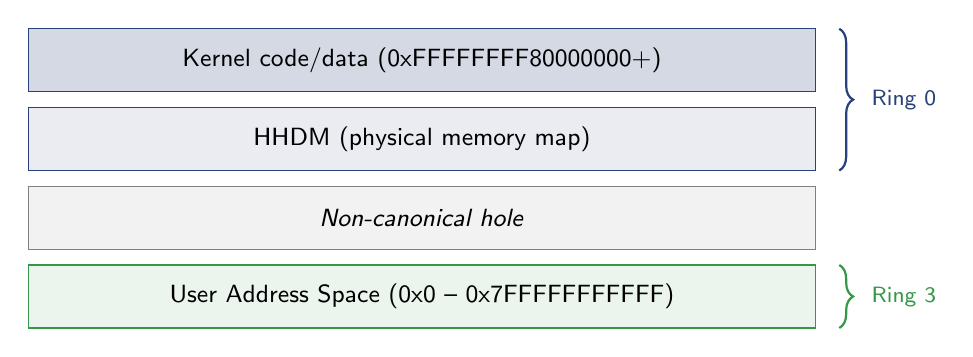
\begin{tikzpicture}[
  every node/.style={font=\sffamily\small},
  region/.style={draw, minimum width=10cm, minimum height=0.8cm, align=center},
  >=Stealth
]

\node[region, fill=user!10, draw=user] (low) at (0, 0) {User Address Space (0x0 -- 0x7FFFFFFFFFFF)};
\node[region, fill=gray!10, draw=gray] (hole) at (0, 1) {\textit{Non-canonical hole}};
\node[region, fill=kernel!10, draw=kernel] (hhdm) at (0, 2) {HHDM (physical memory map)};
\node[region, fill=kernel!20, draw=kernel] (kern) at (0, 3) {Kernel code/data (0xFFFFFFFF80000000+)};

\draw[decorate, decoration={brace, amplitude=5pt, mirror}, thick, kernel]
  (5.3, 1.6) -- (5.3, 3.4)
  node[midway, right=8pt, font=\sffamily\footnotesize, text=kernel] {Ring 0};

\draw[decorate, decoration={brace, amplitude=5pt, mirror}, thick, user]
  (5.3, -0.4) -- (5.3, 0.4)
  node[midway, right=8pt, font=\sffamily\footnotesize, text=user] {Ring 3};

\end{tikzpicture}
\end{center}

% ═════════════════════════════════════════════════════════════════════
\section{IPC in Detail}
% ═════════════════════════════════════════════════════════════════════

\subsection{Syscall Interface}

The entire kernel API is exposed through these syscalls:

\begin{center}
\begin{tabularx}{\textwidth}{llX}
\toprule
\textbf{Number} & \textbf{Syscall} & \textbf{Description} \\
\midrule
0  & \texttt{Yield}          & Yield current timeslice \\
1  & \texttt{Send}           & Send message to endpoint \\
2  & \texttt{Recv}           & Receive message from endpoint \\
3  & \texttt{Call}           & Send + Recv atomically (RPC) \\
\midrule
10 & \texttt{EndpointCreate} & Create new IPC endpoint \\
\midrule
20 & \texttt{FrameAlloc}     & Allocate physical frame \\
21 & \texttt{FrameFree}      & Free physical frame \\
22 & \texttt{Map}            & Map frame into address space \\
23 & \texttt{Unmap}          & Unmap virtual page \\
\midrule
30 & \texttt{CapGrant}       & Delegate capability (with restriction) \\
31 & \texttt{CapRevoke}      & Revoke capability + all derivatives \\
\midrule
40 & \texttt{ThreadCreate}   & Create new thread \\
41 & \texttt{ThreadDestroy}  & Destroy thread \\
\midrule
50 & \texttt{IrqRegister}    & Bind IRQ to endpoint \\
51 & \texttt{IrqAck}         & Acknowledge IRQ \\
\bottomrule
\end{tabularx}
\end{center}

All syscalls require at least one capability as argument.
There is \textbf{no} way to access any resource without the appropriate capability.

\subsection{Typed Channels (Future)}

Each channel will have a schema defined in an Interface Definition Language (IDL).
The IDL compiler generates Rust stubs that serialize/deserialize automatically
with compile-time type checking and zero runtime parsing:

\begin{lstlisting}
// sotos-idl definition (future)
interface FileServer {
    fn open(path: String, flags: u32) -> Result<FileHandle, Error>;
    fn read(handle: FileHandle, buf: &mut [u8]) -> Result<usize, Error>;
    fn write(handle: FileHandle, data: &[u8]) -> Result<usize, Error>;
    fn close(handle: FileHandle) -> Result<(), Error>;
}
\end{lstlisting}

% ═════════════════════════════════════════════════════════════════════
\section{Storage: Transactional Object Store}
% ═════════════════════════════════════════════════════════════════════

Three layers, each providing an escape hatch to the one below:

\begin{center}
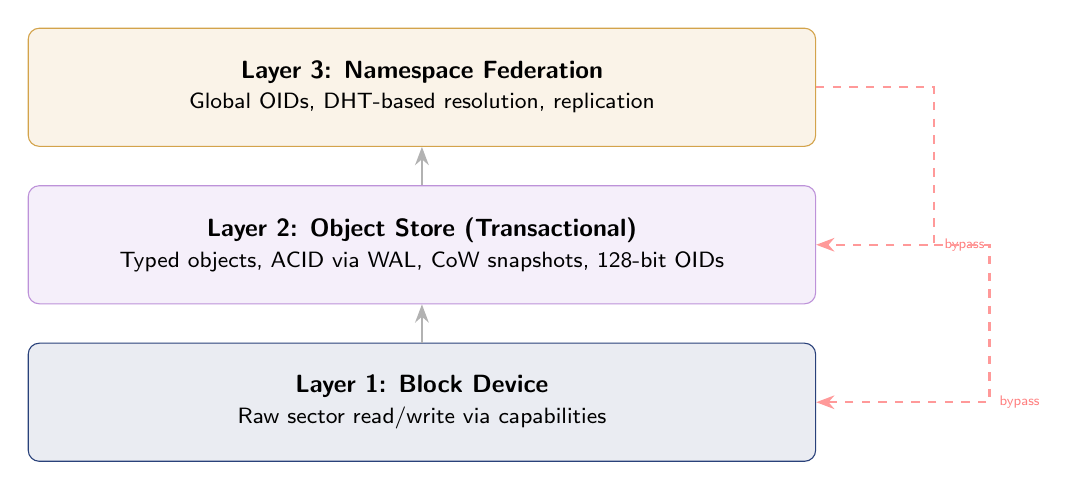
\begin{tikzpicture}[
  every node/.style={font=\sffamily\small},
  layer/.style={draw, rounded corners=4pt, minimum width=10cm, minimum height=1.5cm,
                align=center},
  >=Stealth
]

\node[layer, fill=capcolor!10, draw=capcolor!80] (l3) at (0, 4)
  {\textbf{Layer 3: Namespace Federation}\\
   \footnotesize Global OIDs, DHT-based resolution, replication};

\node[layer, fill=ipc!10, draw=ipc!70] (l2) at (0, 2)
  {\textbf{Layer 2: Object Store (Transactional)}\\
   \footnotesize Typed objects, ACID via WAL, CoW snapshots, 128-bit OIDs};

\node[layer, fill=kernel!10, draw=kernel] (l1) at (0, 0)
  {\textbf{Layer 1: Block Device}\\
   \footnotesize Raw sector read/write via capabilities};

\draw[->, thick, gray!60] (l1) -- (l2);
\draw[->, thick, gray!60] (l2) -- (l3);

\draw[->, thick, red!40, dashed] (l3.east) -- ++(1.5, 0) |- (l2.east)
  node[midway, right, font=\sffamily\tiny, text=red!50] {bypass};
\draw[->, thick, red!40, dashed] (l2.east) ++(1.5,0) -- ++(0.7, 0) |- (l1.east)
  node[midway, right, font=\sffamily\tiny, text=red!50] {bypass};

\end{tikzpicture}
\end{center}

Properties of the Object Store:
\begin{itemize}[leftmargin=2em]
  \item \textbf{Typed objects}: Every object has a schema. No unstructured blobs at this layer.
  \item \textbf{Transactional}: ACID via Write-Ahead Log. Crash at any point $\rightarrow$ consistent recovery.
  \item \textbf{Versioned}: Copy-on-Write at the page level. Every mutation creates an implicit snapshot.
  \item \textbf{POSIX compat}: A translation server can expose the store as a traditional filesystem.
\end{itemize}

% ═════════════════════════════════════════════════════════════════════
\section{Distribution Model}
% ═════════════════════════════════════════════════════════════════════

\subsection{Location Transparency with Explicit Failure}

The same IPC interface works locally and remotely. But remote calls return
\texttt{Result<T, RemoteError>} --- the programmer \textbf{knows} the call can fail
with timeouts, disconnections, and network partitions.

This is fundamentally different from CORBA/DCOM which pretended the network
didn't exist. sotX acknowledges the Fallacies of Distributed Computing.

\subsection{Failure Domain Hierarchy}

\begin{center}
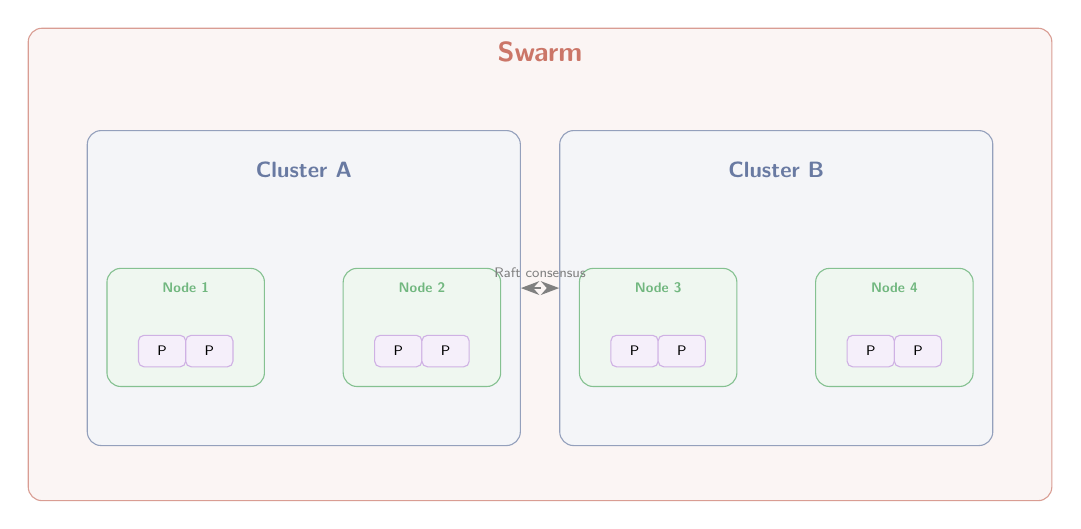
\begin{tikzpicture}[
  every node/.style={font=\sffamily\small},
  domainbox/.style={draw, rounded corners=5pt, align=center},
  >=Stealth
]

\node[domainbox, minimum width=13cm, minimum height=6cm,
      fill=hw!5, draw=hw!50] (swarm) at (0, 0) {};
\node[font=\sffamily\bfseries, text=hw!70] at (0, 2.7) {Swarm};

\node[domainbox, minimum width=5.5cm, minimum height=4cm,
      fill=kernel!5, draw=kernel!50] (c1) at (-3, -0.3) {};
\node[font=\sffamily\bfseries\footnotesize, text=kernel!70] at (-3, 1.2) {Cluster A};

\node[domainbox, minimum width=5.5cm, minimum height=4cm,
      fill=kernel!5, draw=kernel!50] (c2) at (3, -0.3) {};
\node[font=\sffamily\bfseries\footnotesize, text=kernel!70] at (3, 1.2) {Cluster B};

% Nodes in Cluster A
\node[domainbox, minimum width=2cm, minimum height=1.5cm,
      fill=user!8, draw=user!60] (n1) at (-4.5, -0.8) {};
\node[font=\sffamily\tiny\bfseries, text=user!70] at (-4.5, -0.3) {Node 1};
\node[draw=ipc!50, fill=ipc!10, rounded corners=2pt,
      font=\sffamily\tiny, minimum width=0.6cm, minimum height=0.4cm]
  (p1a) at (-4.8, -1.1) {P};
\node[draw=ipc!50, fill=ipc!10, rounded corners=2pt,
      font=\sffamily\tiny, minimum width=0.6cm, minimum height=0.4cm]
  (p1b) at (-4.2, -1.1) {P};

\node[domainbox, minimum width=2cm, minimum height=1.5cm,
      fill=user!8, draw=user!60] (n2) at (-1.5, -0.8) {};
\node[font=\sffamily\tiny\bfseries, text=user!70] at (-1.5, -0.3) {Node 2};
\node[draw=ipc!50, fill=ipc!10, rounded corners=2pt,
      font=\sffamily\tiny, minimum width=0.6cm, minimum height=0.4cm]
  (p2a) at (-1.8, -1.1) {P};
\node[draw=ipc!50, fill=ipc!10, rounded corners=2pt,
      font=\sffamily\tiny, minimum width=0.6cm, minimum height=0.4cm]
  (p2b) at (-1.2, -1.1) {P};

% Nodes in Cluster B
\node[domainbox, minimum width=2cm, minimum height=1.5cm,
      fill=user!8, draw=user!60] (n3) at (1.5, -0.8) {};
\node[font=\sffamily\tiny\bfseries, text=user!70] at (1.5, -0.3) {Node 3};
\node[draw=ipc!50, fill=ipc!10, rounded corners=2pt,
      font=\sffamily\tiny, minimum width=0.6cm, minimum height=0.4cm]
  at (1.2, -1.1) {P};
\node[draw=ipc!50, fill=ipc!10, rounded corners=2pt,
      font=\sffamily\tiny, minimum width=0.6cm, minimum height=0.4cm]
  at (1.8, -1.1) {P};

\node[domainbox, minimum width=2cm, minimum height=1.5cm,
      fill=user!8, draw=user!60] (n4) at (4.5, -0.8) {};
\node[font=\sffamily\tiny\bfseries, text=user!70] at (4.5, -0.3) {Node 4};
\node[draw=ipc!50, fill=ipc!10, rounded corners=2pt,
      font=\sffamily\tiny, minimum width=0.6cm, minimum height=0.4cm]
  at (4.2, -1.1) {P};
\node[draw=ipc!50, fill=ipc!10, rounded corners=2pt,
      font=\sffamily\tiny, minimum width=0.6cm, minimum height=0.4cm]
  at (4.8, -1.1) {P};

% Inter-cluster link
\draw[<->, thick, dashed, gray] (c1.east) -- (c2.west)
  node[midway, above, font=\sffamily\tiny] {Raft consensus};

\end{tikzpicture}
\end{center}

Each level has its own failure detection and recovery:

\begin{center}
\begin{tabularx}{\textwidth}{lXl}
\toprule
\textbf{Level} & \textbf{Failure} & \textbf{Recovery} \\
\midrule
Process & Crash or misbehavior & Restart in milliseconds \\
Node & Hardware failure & Migrate services to another node \\
Cluster & Network partition & Operate in partitioned mode (eventual consistency) \\
Swarm & Cluster disconnect & Autonomous operation, reconcile on reconnect \\
\bottomrule
\end{tabularx}
\end{center}

% ═════════════════════════════════════════════════════════════════════
\section{Boot Chain \& Trust}
% ═════════════════════════════════════════════════════════════════════

\begin{center}
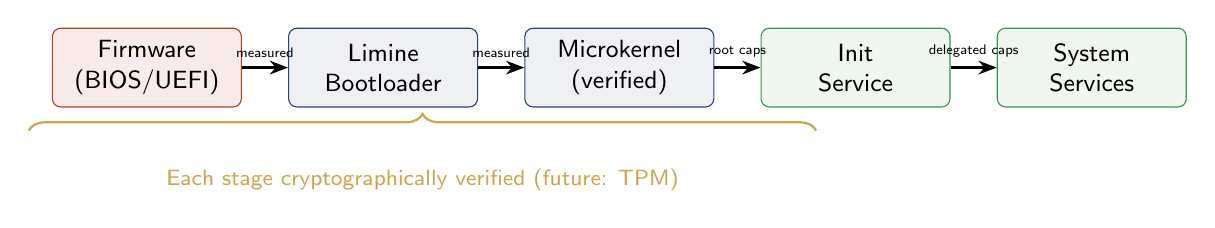
\begin{tikzpicture}[
  every node/.style={font=\sffamily\small},
  stagebox/.style={draw=kernel, fill=kernel!8, rounded corners=3pt,
                minimum width=2.4cm, minimum height=1cm, align=center},
  >=Stealth
]

\node[stagebox, fill=hw!10, draw=hw] (fw) at (0, 0) {Firmware\\(BIOS/UEFI)};
\node[stagebox] (bl) at (3, 0) {Limine\\Bootloader};
\node[stagebox] (kern) at (6, 0) {Microkernel\\(verified)};
\node[stagebox, fill=user!8, draw=user] (init) at (9, 0) {Init\\Service};
\node[stagebox, fill=user!8, draw=user] (svcs) at (12, 0) {System\\Services};

\draw[->, thick] (fw) -- (bl) node[midway, above, font=\sffamily\tiny] {measured};
\draw[->, thick] (bl) -- (kern) node[midway, above, font=\sffamily\tiny] {measured};
\draw[->, thick] (kern) -- (init) node[midway, above, font=\sffamily\tiny] {root caps};
\draw[->, thick] (init) -- (svcs) node[midway, above, font=\sffamily\tiny] {delegated caps};

\draw[decorate, decoration={brace, amplitude=6pt}, thick, capcolor!80]
  (-1.5, -0.8) -- (8.5, -0.8)
  node[midway, below=10pt, font=\sffamily\footnotesize, text=capcolor!80]
  {Each stage cryptographically verified (future: TPM)};

\end{tikzpicture}
\end{center}

The init service is the \textbf{only} process that receives root capabilities.
All other services receive a restricted subset --- the Principle of Least Authority (POLA).

% ═════════════════════════════════════════════════════════════════════
\section{Current Implementation Status}
% ═════════════════════════════════════════════════════════════════════

\subsection{Project Structure}

\begin{center}
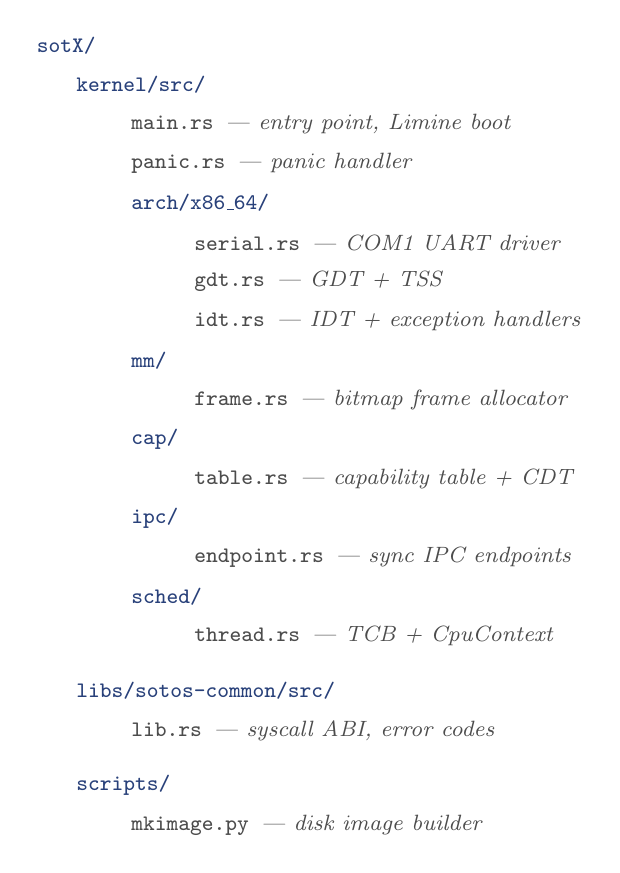
\begin{tikzpicture}[
  every node/.style={font=\ttfamily\footnotesize, anchor=west},
  dir/.style={font=\ttfamily\footnotesize\bfseries, text=kernel},
  file/.style={font=\ttfamily\footnotesize, text=black!70},
]

\node[dir] (root) at (0, 0) {sotX/};
\node[dir] at (0.5, -0.5) {kernel/src/};
\node[file] at (1.2, -1.0) {main.rs \textnormal{\textit{--- entry point, Limine boot}}};
\node[file] at (1.2, -1.5) {panic.rs \textnormal{\textit{--- panic handler}}};
\node[dir] at (1.2, -2.0) {arch/x86\_64/};
\node[file] at (2.0, -2.5) {serial.rs \textnormal{\textit{--- COM1 UART driver}}};
\node[file] at (2.0, -3.0) {gdt.rs \textnormal{\textit{--- GDT + TSS}}};
\node[file] at (2.0, -3.5) {idt.rs \textnormal{\textit{--- IDT + exception handlers}}};
\node[dir] at (1.2, -4.0) {mm/};
\node[file] at (2.0, -4.5) {frame.rs \textnormal{\textit{--- bitmap frame allocator}}};
\node[dir] at (1.2, -5.0) {cap/};
\node[file] at (2.0, -5.5) {table.rs \textnormal{\textit{--- capability table + CDT}}};
\node[dir] at (1.2, -6.0) {ipc/};
\node[file] at (2.0, -6.5) {endpoint.rs \textnormal{\textit{--- sync IPC endpoints}}};
\node[dir] at (1.2, -7.0) {sched/};
\node[file] at (2.0, -7.5) {thread.rs \textnormal{\textit{--- TCB + CpuContext}}};

\node[dir] at (0.5, -8.2) {libs/sotos-common/src/};
\node[file] at (1.2, -8.7) {lib.rs \textnormal{\textit{--- syscall ABI, error codes}}};

\node[dir] at (0.5, -9.4) {scripts/};
\node[file] at (1.2, -9.9) {mkimage.py \textnormal{\textit{--- disk image builder}}};

\end{tikzpicture}
\end{center}

\subsection{What Works Today}

\begin{center}
\begin{tabularx}{\textwidth}{lXc}
\toprule
\textbf{Component} & \textbf{Status} & \textbf{} \\
\midrule
Limine boot (BIOS)         & Kernel loads and executes           & \textcolor{green!60!black}{\cmark} \\
Serial output              & COM1 UART, \texttt{kprintln!} macro & \textcolor{green!60!black}{\cmark} \\
GDT + TSS                  & 64-bit segments, double fault IST   & \textcolor{green!60!black}{\cmark} \\
IDT                        & Breakpoint, double fault, GPF, PF   & \textcolor{green!60!black}{\cmark} \\
Frame allocator            & Bitmap, alloc/free, HHDM            & \textcolor{green!60!black}{\cmark} \\
Capability table           & Insert, lookup, CDT revocation      & \textcolor{green!60!black}{\cmark} \\
IPC endpoints              & Create only (no send/recv yet)       & \textcolor{yellow!60!black}{$\sim$} \\
Scheduler                  & TCB defined (no context switch yet) & \textcolor{yellow!60!black}{$\sim$} \\
Syscall ABI                & Defined in sotos-common             & \textcolor{yellow!60!black}{$\sim$} \\
QEMU boot pipeline         & \texttt{just run} end-to-end        & \textcolor{green!60!black}{\cmark} \\
\midrule
Timer interrupt            & Not implemented                     & \textcolor{red!60}{\xmark} \\
Context switching          & Not implemented                     & \textcolor{red!60}{\xmark} \\
Syscall entry/exit         & Not implemented                     & \textcolor{red!60}{\xmark} \\
Ring 3 (userspace)         & Not implemented                     & \textcolor{red!60}{\xmark} \\
Shared-memory channels     & Not implemented                     & \textcolor{red!60}{\xmark} \\
VMM server                 & Not implemented                     & \textcolor{red!60}{\xmark} \\
\bottomrule
\end{tabularx}
\end{center}

\subsection{Boot Output}

When the kernel boots in QEMU, the serial output shows:

\begin{lstlisting}[style=rust, numbers=none, frame=single, backgroundcolor=\color{black!90},
  basicstyle=\ttfamily\small\color{green!70}]
limine: Loading executable `boot():/boot/sotos-kernel`...
sotX v0.1.0 -- microkernel booting...
[ok] GDT
[ok] IDT
  frames: 268435456 total, 55982 free (218 MiB usable)
[ok] Frame allocator
  capability table ready (max 4096 entries)
[ok] Capabilities
  scheduler: preemptive round-robin (single core)
[ok] Scheduler
Kernel ready. Primitives: sched, irq, ipc, cap, frame_alloc
Halting -- no init service yet.
\end{lstlisting}

% ═════════════════════════════════════════════════════════════════════
\section{Comparison with Existing Systems}
% ═════════════════════════════════════════════════════════════════════

\begin{center}
\begin{tabularx}{\textwidth}{l *{4}{>{\centering\arraybackslash}X}}
\toprule
\textbf{Property} & \textbf{Legacy UNIX} & \textbf{seL4} & \textbf{Fuchsia} & \textbf{sotX} \\
\midrule
Architecture      & Monolithic     & Microkernel    & Microkernel      & Micro + exo bypass \\
Language          & C              & C + Isabelle   & C++ / Rust       & Rust + Verus \\
Verification      & No             & Full proof     & Partial          & Target: full \\
VM in kernel      & Yes            & Yes            & Yes              & \textbf{No} (userspace) \\
Capabilities      & No (DAC/MAC)   & Yes            & Yes (handles)    & Yes + CHERI \\
IPC               & Pipes/sockets  & Sync endpoints & Channels         & Endpoints + channels \\
Zero-copy         & splice/io\_uring & No            & VMOs             & Ring buffers \\
Scheduling        & CFS/RT         & Fixed priority & Fair scheduler   & Hierarchical + domains \\
POSIX compat      & Native         & Manual         & Starnix layer    & \textbf{LUCAS} \\
\bottomrule
\end{tabularx}
\end{center}

% ═════════════════════════════════════════════════════════════════════
\section{Observability}
% ═════════════════════════════════════════════════════════════════════

Every service in sotX exposes metrics and traces natively:

\begin{itemize}[leftmargin=2em]
  \item \textbf{Distributed tracing}: Every IPC message carries a trace ID.
        A request can be traced across N services end-to-end.
  \item \textbf{Metrics}: Counters, histograms, gauges in a standard format.
        The system aggregates automatically.
  \item \textbf{Audit log}: Every capability invocation can be logged,
        creating a complete forensic trail.
\end{itemize}

\begin{center}
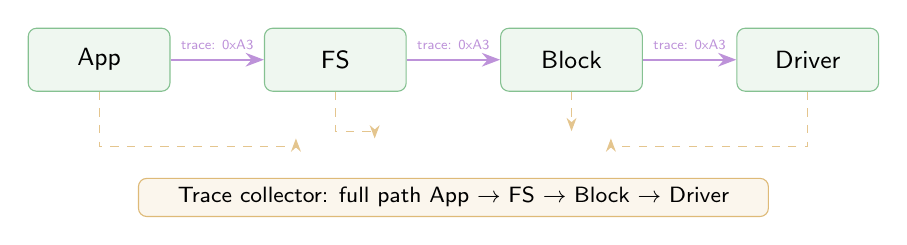
\begin{tikzpicture}[
  every node/.style={font=\sffamily\small},
  svc/.style={draw=user!60, fill=user!8, rounded corners=3pt,
              minimum width=1.8cm, minimum height=0.8cm, align=center},
  >=Stealth
]

\node[svc] (app) at (0, 0) {App};
\node[svc] (fs) at (3, 0) {FS};
\node[svc] (blk) at (6, 0) {Block};
\node[svc] (drv) at (9, 0) {Driver};

\draw[->, thick, ipc!70] (app) -- (fs) node[midway, above, font=\sffamily\tiny] {trace: 0xA3};
\draw[->, thick, ipc!70] (fs) -- (blk) node[midway, above, font=\sffamily\tiny] {trace: 0xA3};
\draw[->, thick, ipc!70] (blk) -- (drv) node[midway, above, font=\sffamily\tiny] {trace: 0xA3};

\node[draw=capcolor!60, fill=capcolor!8, rounded corners=3pt, below=1cm,
      minimum width=8cm, font=\sffamily\footnotesize] at (4.5, -0.5)
  {Trace collector: full path App $\rightarrow$ FS $\rightarrow$ Block $\rightarrow$ Driver};

\draw[->, dashed, capcolor!50] (app.south) -- ++(0, -0.7) -| (2.5, -1.0);
\draw[->, dashed, capcolor!50] (fs.south) -- ++(0, -0.5) -| (3.5, -1.0);
\draw[->, dashed, capcolor!50] (blk.south) -- ++(0, -0.5);
\draw[->, dashed, capcolor!50] (drv.south) -- ++(0, -0.7) -| (6.5, -1.0);

\end{tikzpicture}
\end{center}

% ═════════════════════════════════════════════════════════════════════
\section{Hot-Patching \& Live Update}
% ═════════════════════════════════════════════════════════════════════

Userspace services can be updated without system restart:

\begin{center}
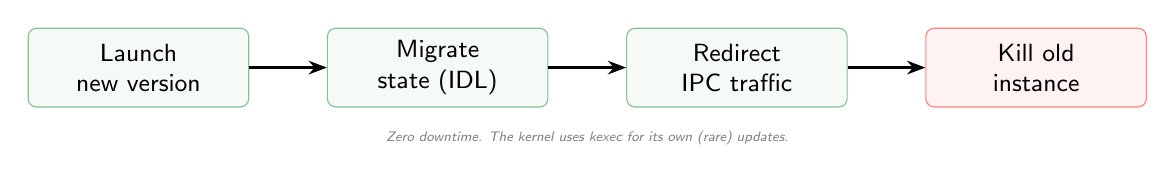
\begin{tikzpicture}[
  every node/.style={font=\sffamily\small},
  stepbox/.style={draw=user!60, fill=user!5, rounded corners=3pt,
               minimum width=2.8cm, minimum height=1cm, align=center},
  >=Stealth
]

\node[stepbox] (s1) at (0, 0) {Launch\\new version};
\node[stepbox] (s2) at (3.8, 0) {Migrate\\state (IDL)};
\node[stepbox] (s3) at (7.6, 0) {Redirect\\IPC traffic};
\node[stepbox, draw=red!50, fill=red!5] (s4) at (11.4, 0) {Kill old\\instance};

\draw[->, thick] (s1) -- (s2);
\draw[->, thick] (s2) -- (s3);
\draw[->, thick] (s3) -- (s4);

\node[font=\sffamily\tiny\itshape, text=gray] at (5.7, -0.9)
  {Zero downtime. The kernel uses kexec for its own (rare) updates.};

\end{tikzpicture}
\end{center}

% ═════════════════════════════════════════════════════════════════════
\section{LUCAS: Legacy UNIX Compatibility Abstraction System}
% ═════════════════════════════════════════════════════════════════════

LUCAS is a userspace subsystem that allows \textbf{unmodified Linux/POSIX ELF binaries}
to run natively on sotX. Unlike a hypervisor that virtualizes hardware,
LUCAS is a \textit{paravirtualizer of interfaces} --- it translates monolithic
UNIX semantics into sotX's decentralized, capability-based primitives.

\begin{principalbox}{LUCAS in One Sentence}
LUCAS presents the illusion of a complete Linux system to legacy binaries,
while every operation is actually mediated by capabilities and sotX IPC
underneath. The guest binary thinks it's on Linux; it's actually sandboxed
in a capability jail.
\end{principalbox}

\subsection{Architecture}

LUCAS is not a monolithic emulator --- it is a set of coordinated Ring~3 servers:

\begin{center}
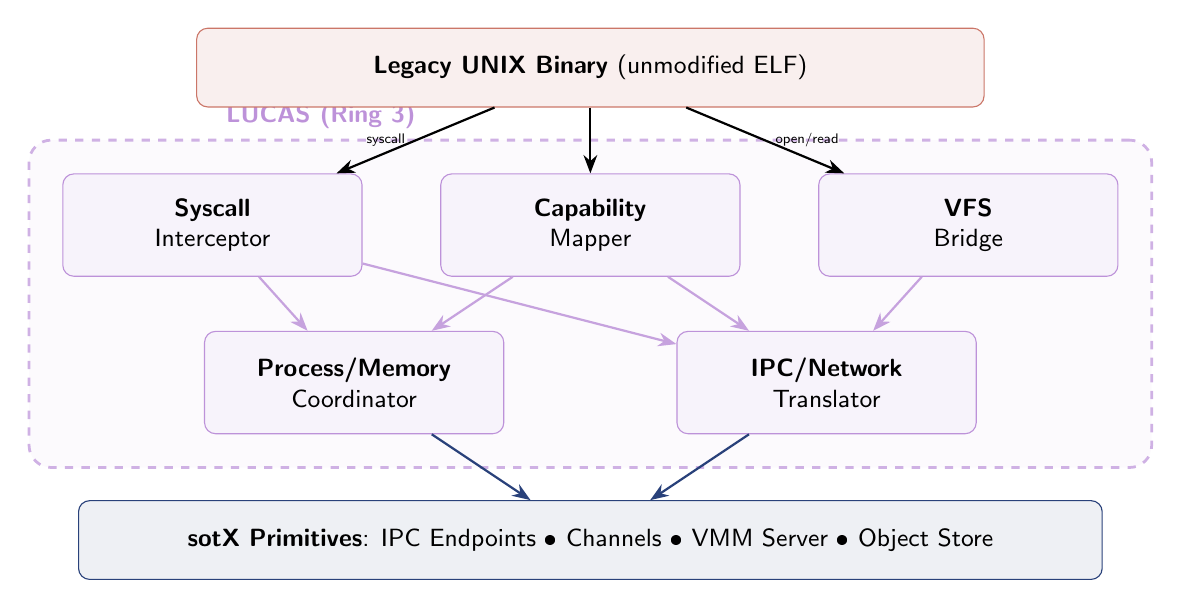
\begin{tikzpicture}[
  every node/.style={font=\sffamily\small},
  comp/.style={draw=ipc!70, fill=ipc!8, rounded corners=4pt,
               minimum width=3.8cm, minimum height=1.3cm, align=center},
  elf/.style={draw=hw!70, fill=hw!8, rounded corners=4pt,
              minimum width=10cm, minimum height=1cm, align=center},
  kern/.style={draw=kernel, fill=kernel!8, rounded corners=4pt,
               minimum width=13cm, minimum height=1cm, align=center},
  >=Stealth
]

% ELF binary
\node[elf] (binary) at (0, 6.5)
  {\textbf{Legacy UNIX Binary} (unmodified ELF)};

% LUCAS components
\node[comp] (trap) at (-4.8, 4.5) {\textbf{Syscall}\\Interceptor};
\node[comp] (capmap) at (0, 4.5) {\textbf{Capability}\\Mapper};
\node[comp] (vfs) at (4.8, 4.5) {\textbf{VFS}\\Bridge};

\node[comp] (proc) at (-3, 2.5) {\textbf{Process/Memory}\\Coordinator};
\node[comp] (ipctr) at (3, 2.5) {\textbf{IPC/Network}\\Translator};

% LUCAS boundary
\begin{scope}[on background layer]
\node[draw=ipc!50, fill=ipc!3, rounded corners=8pt, dashed, line width=1pt,
      fit=(trap)(capmap)(vfs)(proc)(ipctr),
      inner sep=12pt, label={[font=\sffamily\bfseries\small, text=ipc!70]
      above left:LUCAS (Ring 3)}] (lucas) {};
\end{scope}

% sotX services
\node[kern] (sotos) at (0, 0.5)
  {\textbf{sotX Primitives}: IPC Endpoints \textbullet{} Channels \textbullet{}
   VMM Server \textbullet{} Object Store};

% Arrows
\draw[->, thick] (binary) -- (trap) node[midway, left, font=\sffamily\tiny] {syscall};
\draw[->, thick] (binary) -- (capmap);
\draw[->, thick] (binary) -- (vfs) node[midway, right, font=\sffamily\tiny] {open/read};

\draw[->, thick, ipc!60] (trap) -- (proc);
\draw[->, thick, ipc!60] (trap) -- (ipctr);
\draw[->, thick, ipc!60] (capmap) -- (proc);
\draw[->, thick, ipc!60] (capmap) -- (ipctr);
\draw[->, thick, ipc!60] (vfs) -- (ipctr);

\draw[->, thick, kernel] (proc) -- (sotos);
\draw[->, thick, kernel] (ipctr) -- (sotos);

\end{tikzpicture}
\end{center}

\subsection{Components}

\begin{center}
\begin{tabularx}{\textwidth}{lX}
\toprule
\textbf{Component} & \textbf{Role} \\
\midrule
\textbf{Syscall Interceptor} &
  Captures \texttt{syscall}/\texttt{int 0x80} from the guest binary in Ring~3.
  Redirects to LUCAS translation engine instead of the kernel.
  Maps Linux syscall numbers to LUCAS handlers. \\
\midrule
\textbf{Capability Mapper} &
  Maintains an internal table mapping Linux file descriptors (FDs) and PIDs
  to real sotX capabilities. Emulates UID/GID permissions on top of the
  capability model. Hides the CDT from the guest binary. \\
\midrule
\textbf{VFS Bridge} &
  Intercepts POSIX file operations (\texttt{open}, \texttt{read}, \texttt{write}, \texttt{stat})
  and translates them to Object Store (Layer~2) transactions.
  Exposes typed objects as flat byte streams. Synthesizes \texttt{/proc} and \texttt{/sys}. \\
\midrule
\textbf{Process/Memory Coordinator} &
  Emulates \texttt{fork()} (CoW via VMM), \texttt{execve()} (ELF parsing + segment mapping),
  \texttt{mmap()}/\texttt{brk()} (delegated to VMM server).
  Creates threads via \texttt{sys\_thread\_create}. \\
\midrule
\textbf{IPC/Network Translator} &
  Translates UNIX pipes $\rightarrow$ ring buffer channels,
  signals $\rightarrow$ endpoint messages,
  sockets $\rightarrow$ channels (zero-copy for high throughput).
  Emulates \texttt{epoll}/\texttt{select} over sotX IPC. \\
\bottomrule
\end{tabularx}
\end{center}

\subsection{Execution Flow: \texttt{write(fd, buf, size)}}

\begin{center}
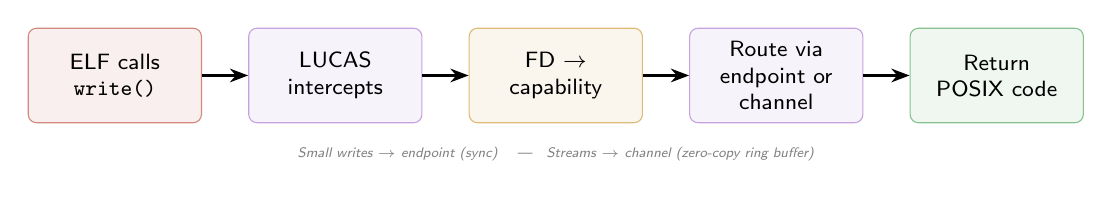
\begin{tikzpicture}[
  every node/.style={font=\sffamily\small},
  flowbox/.style={draw=kernel!60, fill=kernel!5, rounded corners=3pt,
               minimum width=2.2cm, minimum height=1.2cm, align=center,
               font=\sffamily\footnotesize},
  >=Stealth
]

\node[flowbox, fill=hw!8, draw=hw!60] (s1) at (0, 0)
  {ELF calls\\\texttt{write()}};
\node[flowbox, fill=ipc!8, draw=ipc!60] (s2) at (2.8, 0)
  {LUCAS\\intercepts};
\node[flowbox, fill=capcolor!8, draw=capcolor!60] (s3) at (5.6, 0)
  {FD $\rightarrow$\\capability};
\node[flowbox, fill=ipc!8, draw=ipc!60] (s4) at (8.4, 0)
  {Route via\\endpoint or\\channel};
\node[flowbox, fill=user!8, draw=user!60] (s5) at (11.2, 0)
  {Return\\POSIX code};

\draw[->, thick] (s1) -- (s2);
\draw[->, thick] (s2) -- (s3);
\draw[->, thick] (s3) -- (s4);
\draw[->, thick] (s4) -- (s5);

\node[font=\sffamily\tiny\itshape, text=gray] at (5.6, -1.0)
  {Small writes $\rightarrow$ endpoint (sync) \quad|\quad
   Streams $\rightarrow$ channel (zero-copy ring buffer)};

\end{tikzpicture}
\end{center}

\subsection{Security: Confinement by Design}

From a cybersecurity perspective, LUCAS operates as a \textbf{strict isolation sandbox}:

\begin{center}
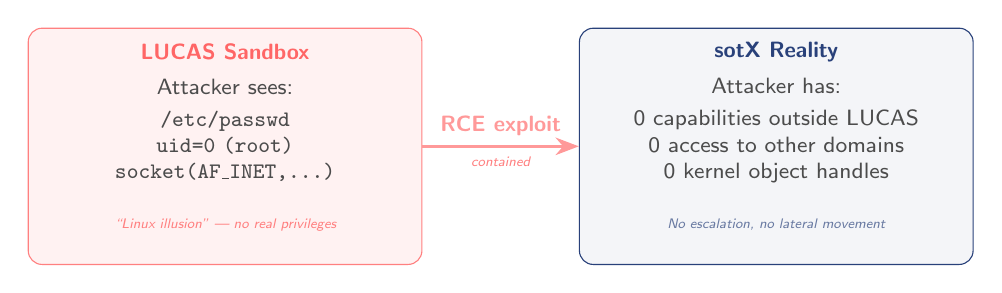
\begin{tikzpicture}[
  every node/.style={font=\sffamily\small},
  >=Stealth
]

% The illusion
\node[draw=red!50, fill=red!5, rounded corners=5pt,
      minimum width=5cm, minimum height=3cm] (jail) at (0, 0) {};
\node[font=\sffamily\bfseries\footnotesize, text=red!60] at (0, 1.2)
  {LUCAS Sandbox};
\node[font=\sffamily\footnotesize, text=black!70, text width=4cm, align=center]
  at (0, 0.2)
  {Attacker sees:\\[2pt]
   \texttt{/etc/passwd}\\
   \texttt{uid=0 (root)}\\
   \texttt{socket(AF\_INET,...)}};
\node[font=\sffamily\tiny\itshape, text=red!50] at (0, -1.0)
  {``Linux illusion'' --- no real privileges};

% The reality
\node[draw=kernel, fill=kernel!5, rounded corners=5pt,
      minimum width=5cm, minimum height=3cm] (real) at (7, 0) {};
\node[font=\sffamily\bfseries\footnotesize, text=kernel] at (7, 1.2)
  {sotX Reality};
\node[font=\sffamily\footnotesize, text=black!70, text width=4cm, align=center]
  at (7, 0.2)
  {Attacker has:\\[2pt]
   0 capabilities outside LUCAS\\
   0 access to other domains\\
   0 kernel object handles};
\node[font=\sffamily\tiny\itshape, text=kernel!70] at (7, -1.0)
  {No escalation, no lateral movement};

% Arrow
\draw[->, very thick, red!40] (jail.east) -- (real.west)
  node[midway, above, font=\sffamily\footnotesize\bfseries] {RCE exploit}
  node[midway, below, font=\sffamily\tiny\itshape, text=red!50] {contained};

\end{tikzpicture}
\end{center}

\begin{warningbox}{Why LUCAS Is Fundamentally More Secure Than Linux}
In sotX, there is \textbf{no ambient authority}. A Linux binary running inside LUCAS
can only interact with resources that LUCAS explicitly provides capabilities for.
Even if an attacker achieves Remote Code Execution (RCE) by exploiting a vulnerability
in an emulated web server, the damage is confined:

\begin{itemize}[leftmargin=1.5em]
  \item The compromised binary holds no native capabilities to interact with other
        sotX protection domains or the underlying hardware.
  \item The attacker is trapped inside the ``Linux illusion'' --- they can corrupt
        the emulated environment but cannot escape the capability jail.
  \item Privilege escalation is structurally impossible: there is no \texttt{root},
        no \texttt{/dev/mem}, no \texttt{CAP\_SYS\_ADMIN} --- only capability tokens
        that the kernel validates on every operation.
\end{itemize}
\end{warningbox}

\subsection{Comparison with Other Compatibility Layers}

\begin{center}
\begin{tabularx}{\textwidth}{l *{4}{>{\centering\arraybackslash}X}}
\toprule
\textbf{Property} & \textbf{WSL1} & \textbf{Wine} & \textbf{Fuchsia Starnix} & \textbf{LUCAS} \\
\midrule
Runs in          & Kernel       & Userspace    & Kernel runner       & Userspace \\
Target ABI       & Linux        & Win32        & Linux               & Linux/POSIX \\
Isolation         & Weak         & None         & Moderate (zircon)   & \textbf{Full (caps)} \\
Zero-copy IPC     & No           & No           & VMOs                & Ring buffers \\
Native perf       & Good         & Variable     & Good                & Good (bypass) \\
Security model    & Shared kernel & Shared proc  & Handles             & Capability jail \\
\bottomrule
\end{tabularx}
\end{center}

% ═════════════════════════════════════════════════════════════════════
\section{Summary: Design Principles}
% ═════════════════════════════════════════════════════════════════════

\begin{center}
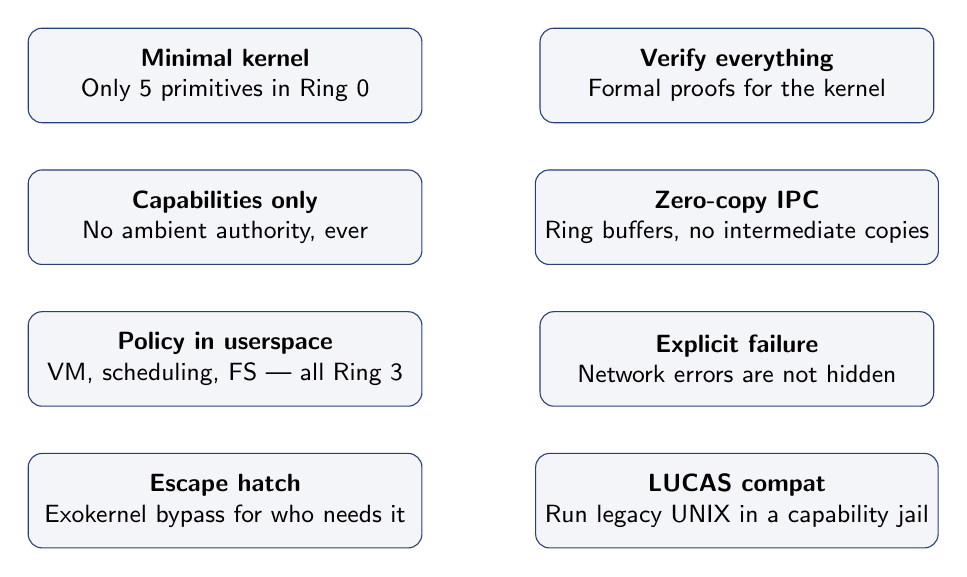
\begin{tikzpicture}[
  every node/.style={font=\sffamily},
  principle/.style={draw=kernel, fill=kernel!5, rounded corners=5pt,
                    minimum width=5cm, minimum height=1.2cm, align=center,
                    font=\sffamily\small},
]

\node[principle] (p1) at (0, 5)   {\textbf{Minimal kernel}\\Only 5 primitives in Ring 0};
\node[principle] (p2) at (6.5, 5) {\textbf{Verify everything}\\Formal proofs for the kernel};
\node[principle] (p3) at (0, 3.2) {\textbf{Capabilities only}\\No ambient authority, ever};
\node[principle] (p4) at (6.5, 3.2) {\textbf{Zero-copy IPC}\\Ring buffers, no intermediate copies};
\node[principle] (p5) at (0, 1.4) {\textbf{Policy in userspace}\\VM, scheduling, FS --- all Ring 3};
\node[principle] (p6) at (6.5, 1.4) {\textbf{Explicit failure}\\Network errors are not hidden};
\node[principle] (p7) at (0, -0.4) {\textbf{Escape hatch}\\Exokernel bypass for who needs it};
\node[principle] (p8) at (6.5, -0.4) {\textbf{LUCAS compat}\\Run legacy UNIX in a capability jail};

\end{tikzpicture}
\end{center}

\vfill

\begin{center}
\rule{0.5\textwidth}{0.4pt}\\[1em]
{\large\sffamily\color{accent} sotX --- The kernel guarantees isolation, not policy.}\\[0.5em]
{\small\sffamily\color{gray} v0.1.0 \textbullet{} March 2026}
\end{center}

\end{document}
